\section{Interface Rank Preservation} \label{section:interface_rank_preservation}

Absolute energy discrepancies were evident but secondary to the study goal. More relevant was the preservation of ranking. For Ge and Sn, MLPs captured the energetic hierarchy of interfaces with reasonable fidelity, while for Si, the energetic ordering was often disrupted.

\begin{figure}[h]
    \centering
    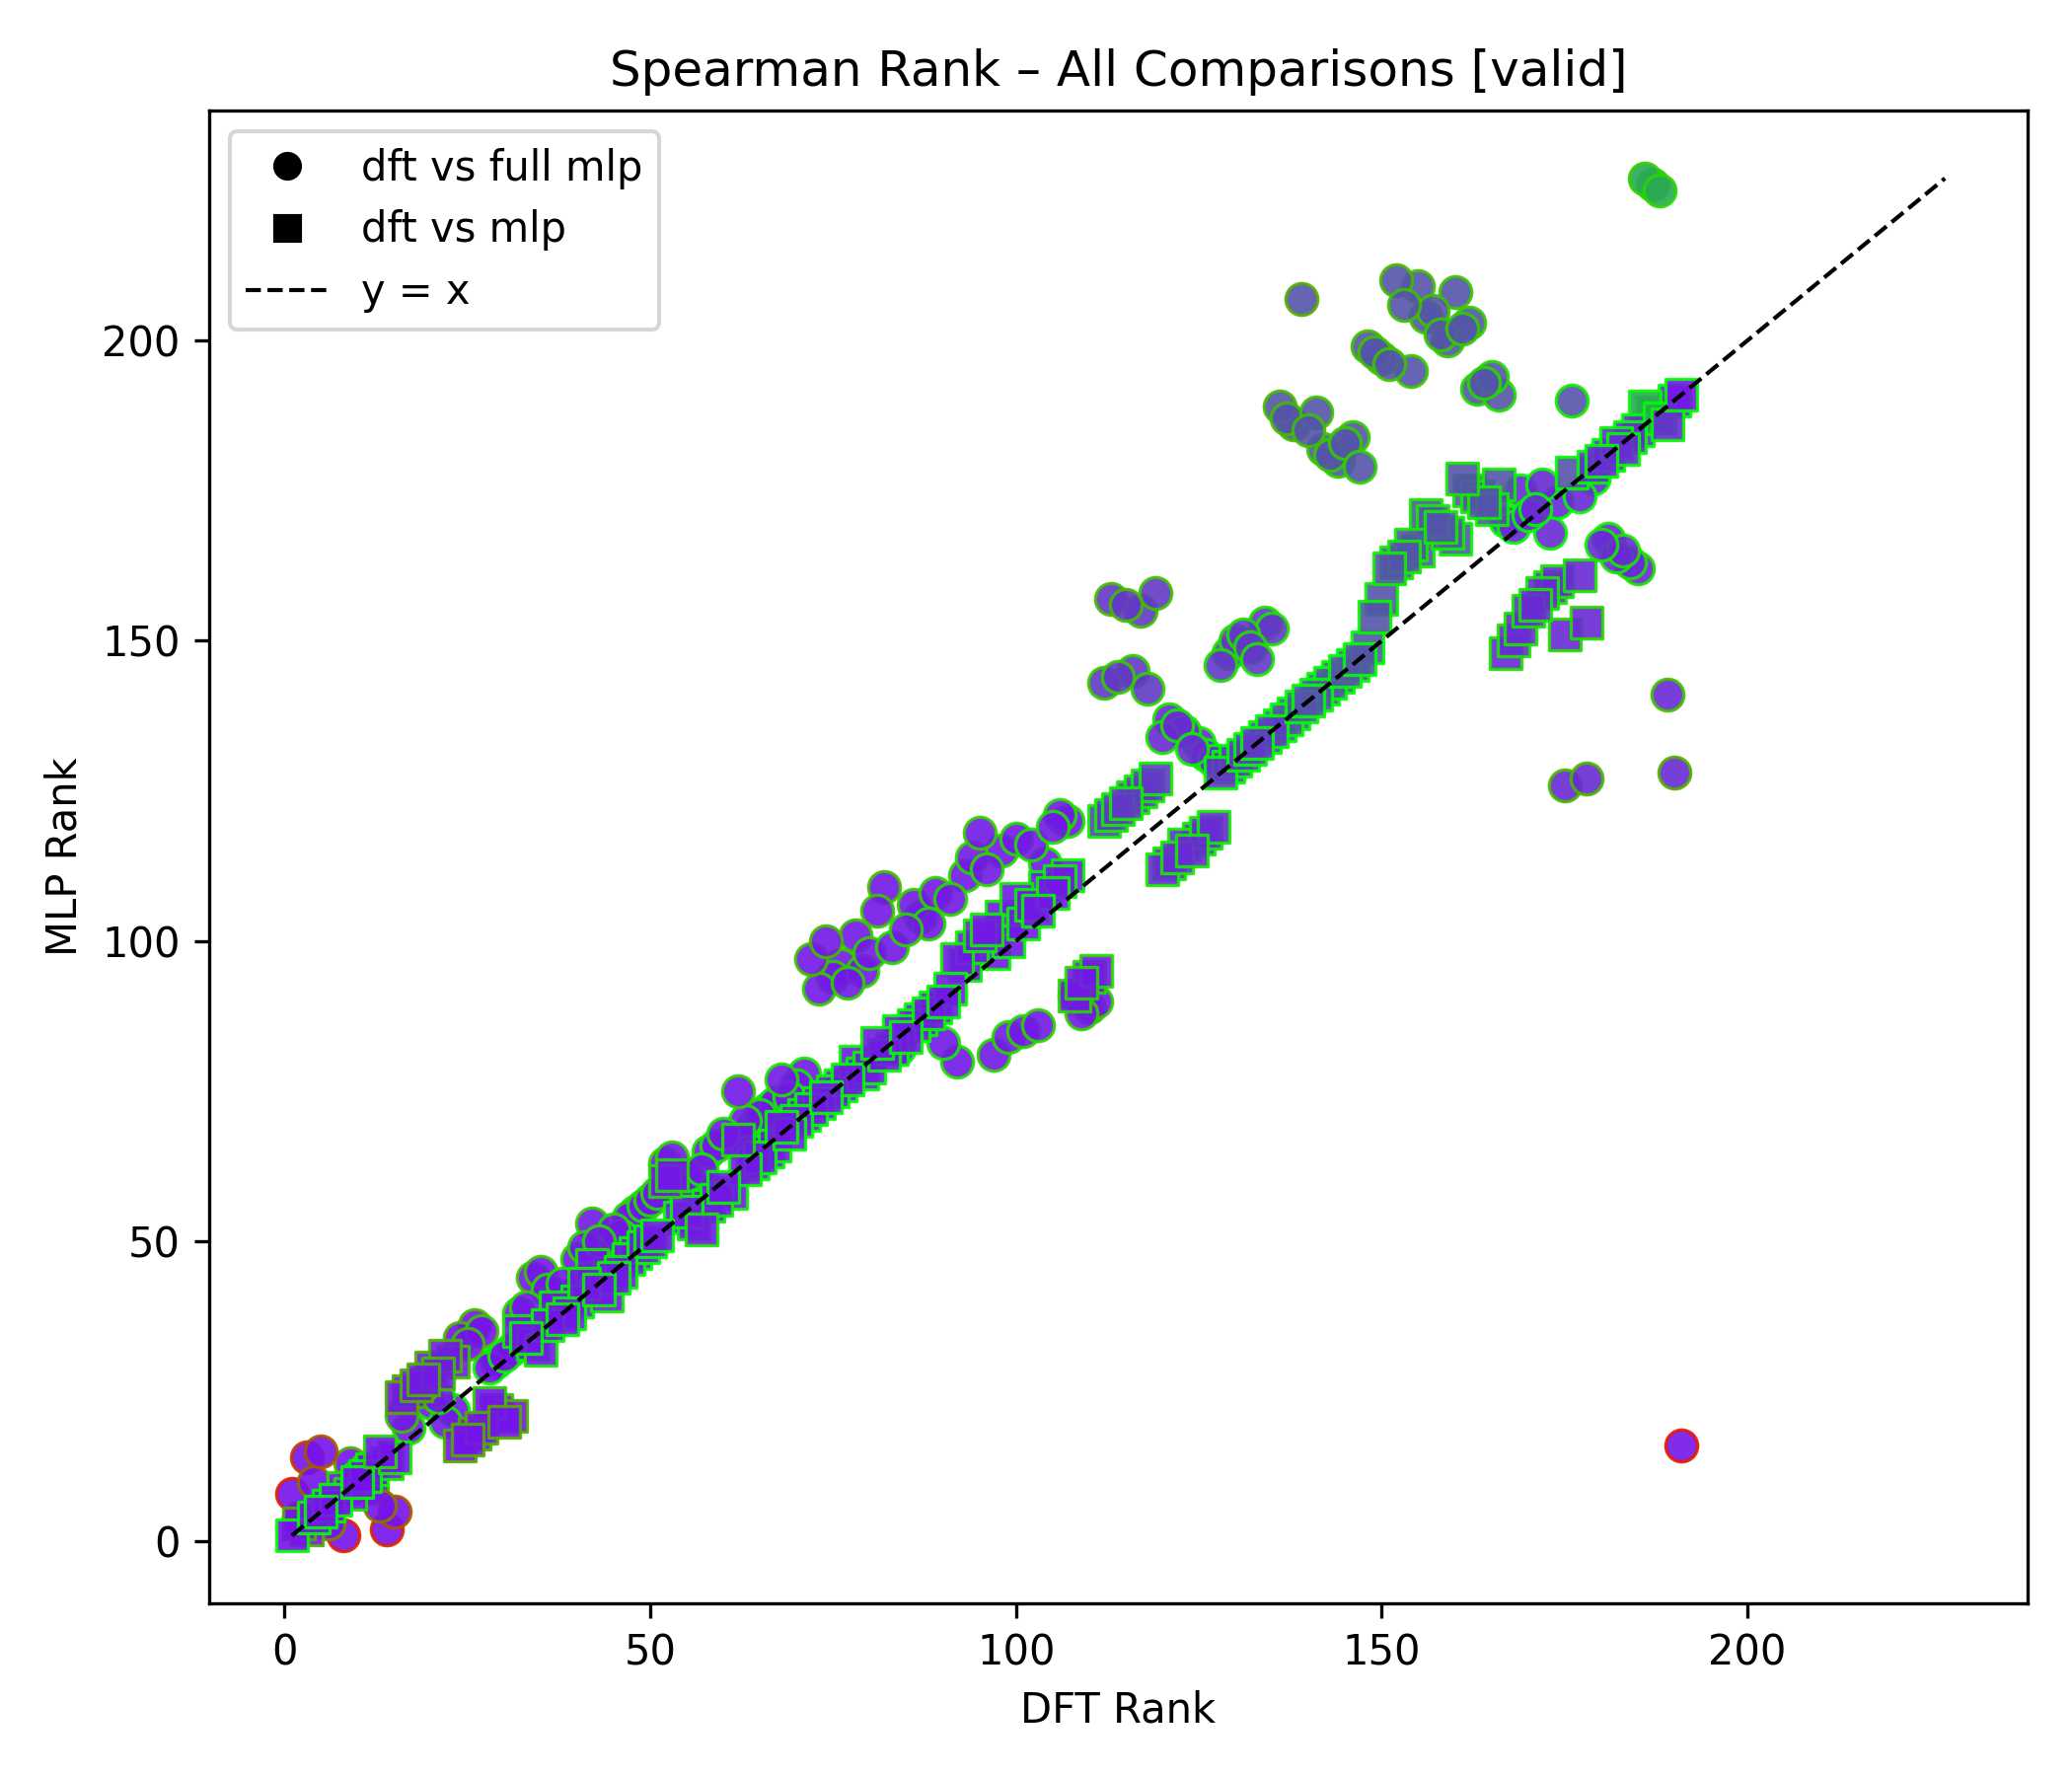
\includegraphics[width=0.7\textwidth]{analysis/plots/results_lower_Ge_spearman_all_comparisons_valid.png}
    \caption{Spearman correlation for Ge interfaces.}
\end{figure}

Top-N overlap and Spearman/Kendall rank statistics highlighted the utility of MLPs in screening contexts. Even where absolute energies were misaligned, the preservation of top candidate rankings proved robust in Ge and Sn systems.

\begin{figure}[h]
    \centering
    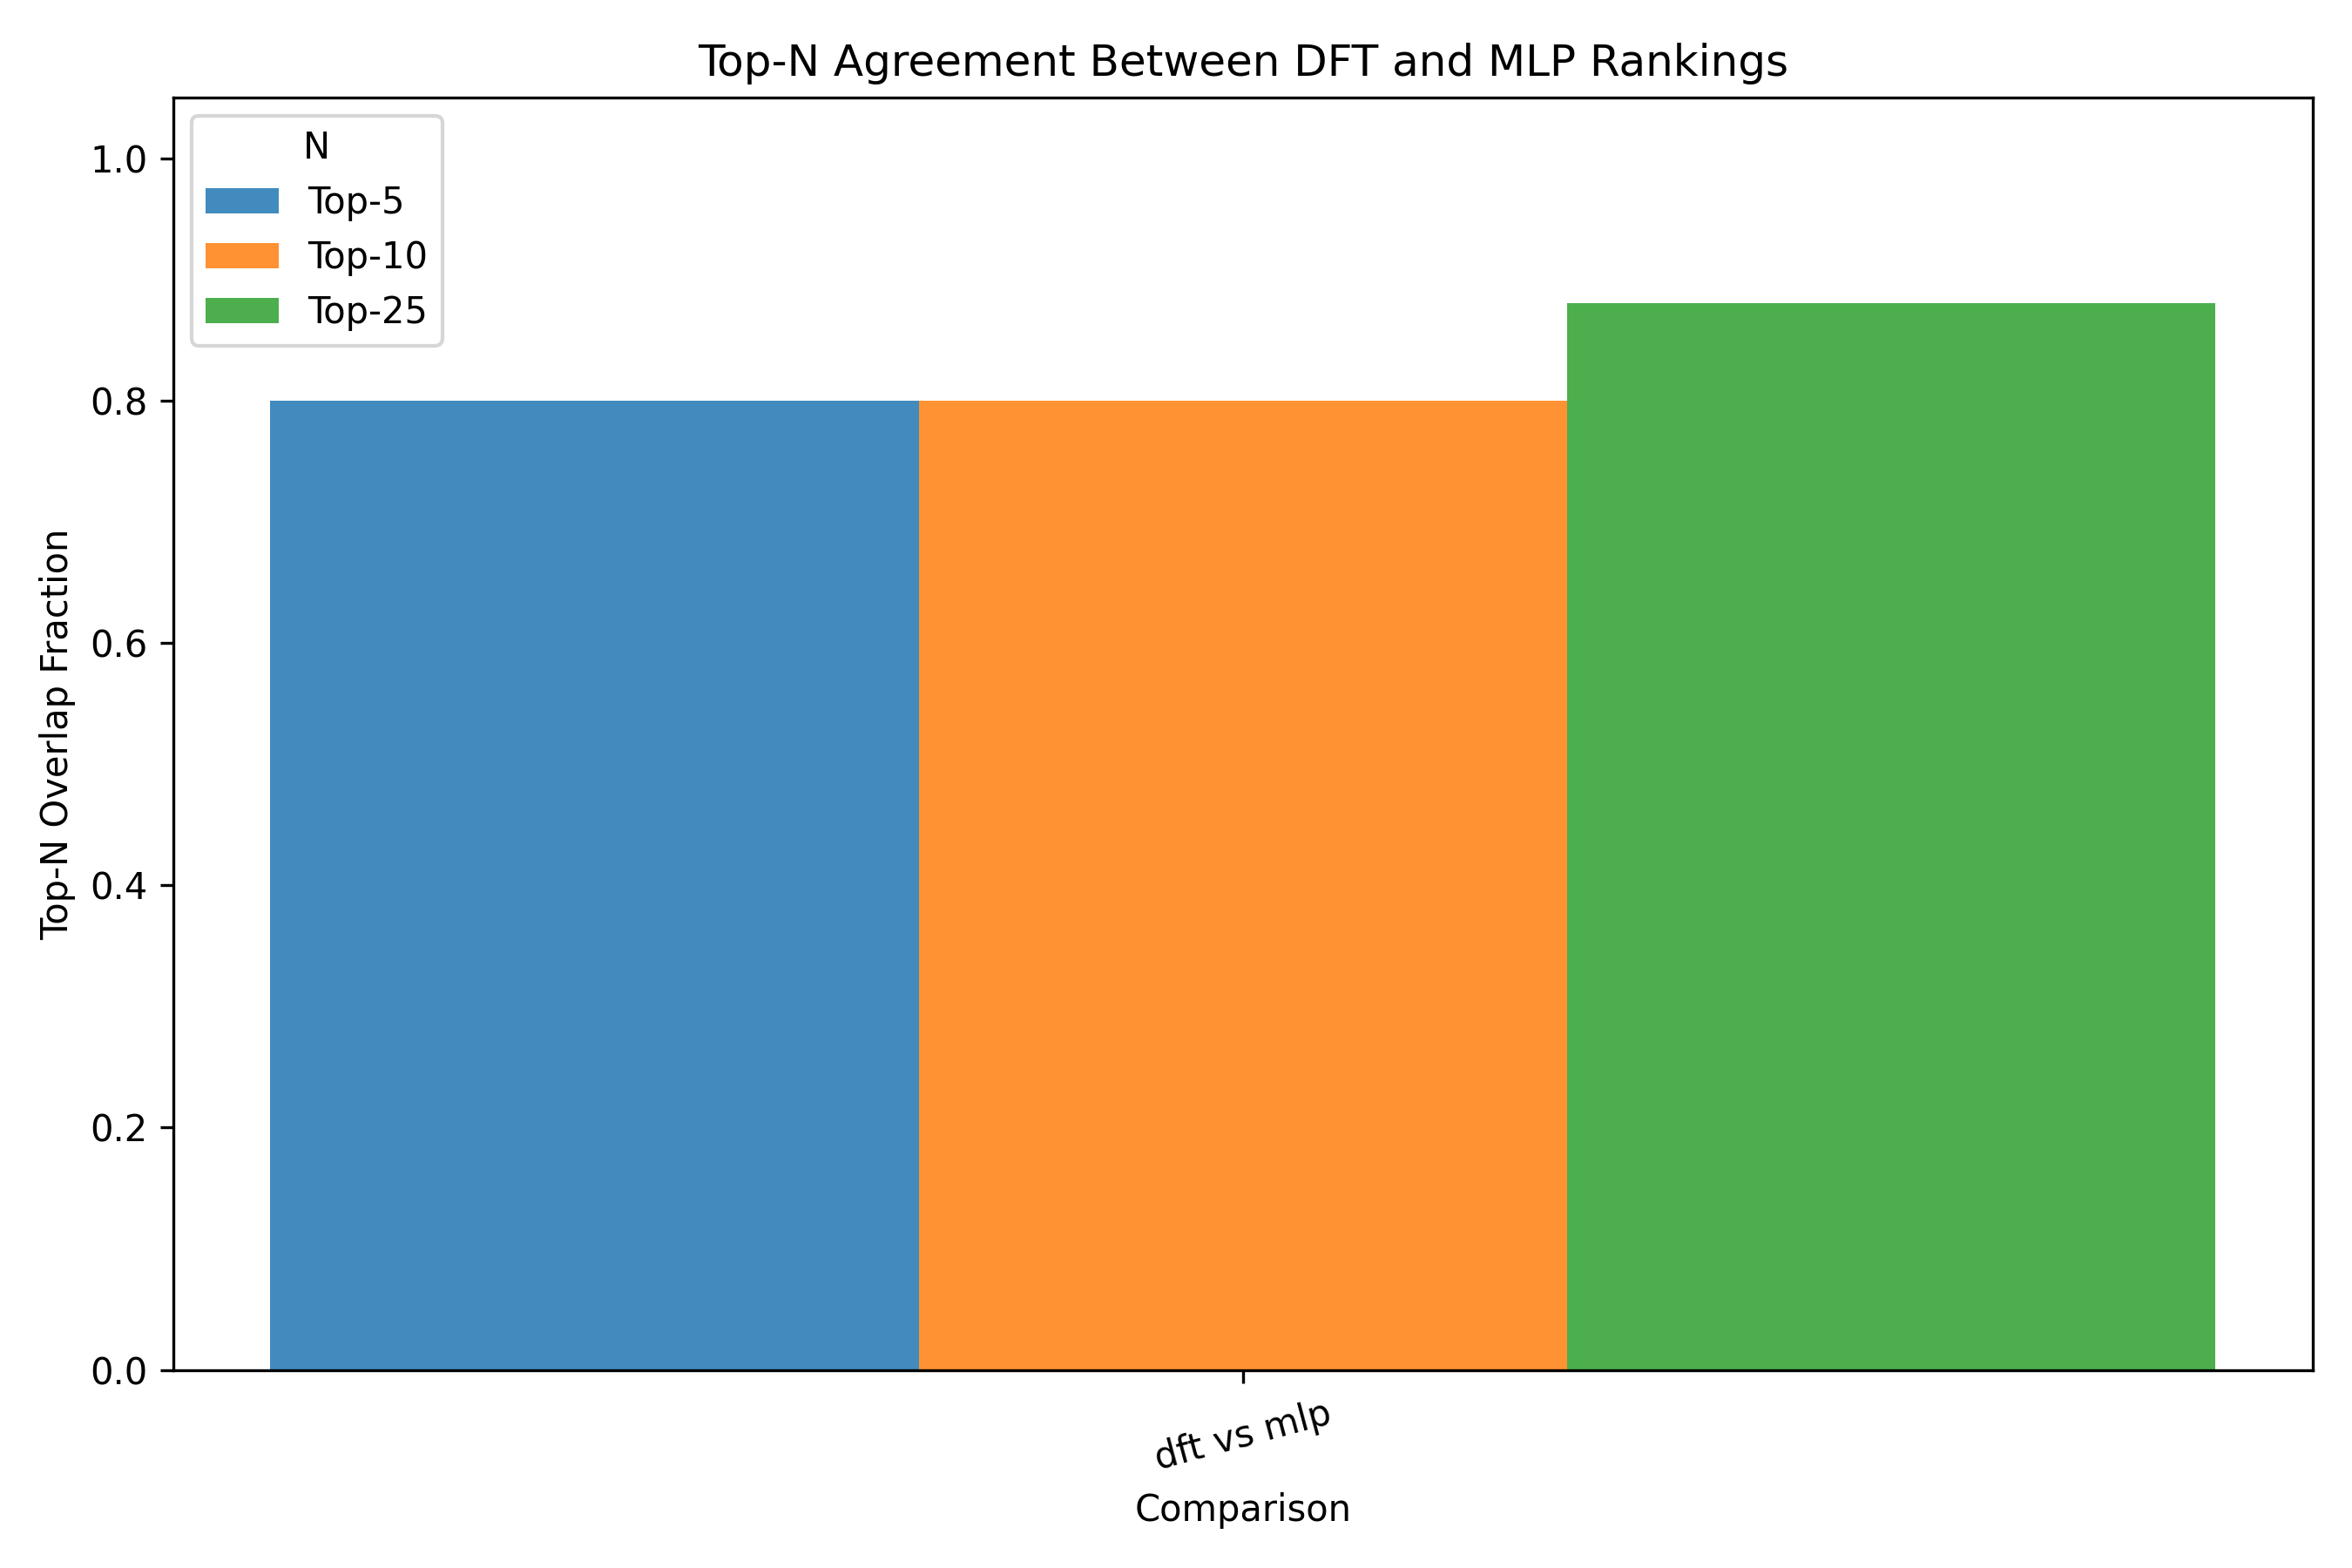
\includegraphics[width=0.7\textwidth]{analysis/plots/results_lower_Si_topn_overlap.png}
    \caption{Top-\textit{N} overlap for Si interfaces.}
\end{figure}

MLPs offer clear advantages in computational speed and can safely be used for preliminary screening in certain systems. However, their generalisation is inconsistent, especially in covalently bonded systems like Si. Without targeted retraining, MLPs may mislead in these cases.

% todo Equation suggestion: O(n) comparison of DFT vs MLP computational cost per electron.